\chapter{ROS}

\section{Overview}
The Robot Operating System (ROS) is a meta operating system for open-source robotics.

It provides package management, an asynchronous messaging framework between processes

All software components in this project communicate using the asynchronous, distributed framework supported by ROS.

\subsection{Nodes}
Processes in ROS are known as nodes.

\subsection{Messages}
Messages are data structures which contain some amount of named data fields.
publishing and subscribing messages

\subsection{Topics}
Messages are published to certain topic names. Processes subscribe to these topic names, and receive all messages sent on those names. Any number of processes may publish or subscribe to a topic, making this a many-to-many communication protocol.

The ROS Master acts like a DNS server, giving nodes references to each other. Let's use an example. Assume node A starts publishing messages to topic "/foo". When node A begins publishing, it will register that fact with the ROS master. If node B wants to subscribe to that same topic, it will communicate its intent to the ROS master. The master will then go through its list of all publishers to that topic, and inform them of node B's desire. In this case, node A is the only publisher, so the master will tell node A what TCP/IP socket to send its data to when it publishes to the "/foo" topic. From then on, when node A publishes a message to "/foo", it will go through its list of nodes subscribed to it, and send a copy of its message to each of those sockets.

Running nodes create a graph based on which nodes send data to which other nodes.

\subsection{Packages}
Packages are collections of related ROS resources to perform some function. They often include node source code, built executables, message definitions, and launch files.

There are also meta-packages which are, simply enough, collections of related packages.

\subsection{Launch Files}
Launch files are simply XML files which define several nodes to be run at the same time. Robotics systems grow large quickly, and dozens of nodes may need to be run to perform some task. Manually starting all of those nodes would be tedious, and launch files save that time. They also allow easy configuration and parameter specification for each node. Parameters are often stored separately in files using the YAML syntax, and loaded dynamically into the launch files. This allows one to bring a node up or down simply by modifying a launch file, but never losing all of the configuration settings for that node.

\subsection{Frames}
Frames are a set of reference coordinate axes.

A common starting frame is the base\_link frame, which has its origin at the center of a robotic chassis. The x-axis of the base\_link frame points forward, the y-axis points to the robot's left, and the z-axis goes straight up above the robot.


position and orientation
quaternion vectors represent orientation
messages have frame\_ids detailing which frame they are in

\subsection{Transforms}
conversions between frames
handled by the ROS package tf
broadcasting transforms


\subsection{User defined packages}
auto\_rover package
Defines launch files, configuration files, message definition for EncCount, and a single range\_converter node. 


\section{rosserial} \label{sectionRosSerial}
Communication between the Arduino and laptop is handled with the ROS metapackage rosserial. Different client packages support different client machines, such as embedded linux devices, or different microcontroller boards. These client packages create local support libraries or header files on those machines, which use a serialization protocol to send and receive ROS messages over a serial port. On the other side of the serial connection, host packages run a bridging node which communicates with the ROS network on behalf of the client machine. Subscribed topics have their messages serialized and sent to the client machine, and outgoing messages from the client are de-serialized and published. 

\subsection{rosserial\_arduino}
rosserial\_arduino is one client package of rosserial, which creates an Arduino library to provide bare-bones ROS support to sketches. The sketch running on this project's Uno board uses this library to publish sensor data as messages, and subscribe to motor command topics.

Every time the sketch wishes to update the laptop with its newest sensor readings, it publishes three messages. First the servo angle in degrees is published to the "/ping/angleDeg" topic, as a standard Int8 message. This message just contains a single data field: an 8-bit signed integer. Next the echo time in microseconds is published to the "/ping/timeUS" topic, as a standard UInt16 message which contains a single 16 bit data field representing an unsigned integer. Lastly the two encoder tick counts are both placed into a single custom message called EncCount, and published to the "/odom/encTicks" topic. This custom message type has two 32 bit fields, one for each encoder. This message type will be further explained in section \ref{sectionEncCount}.

When the sketch is waiting between updates, it continually listens to the serial port for motor commands. These commands are Int8 messages on the "/cmd/left" or "/cmd/right" topics, which the sketch subscribes to. When these messages are found in the serial input buffer, a short callback function is executed, which writes the R/C pulse command to the proper motor channel.

Arduino boards use different types of memory. Flash memory is used to store sketch code, and static random access memory (SRAM) is used to store dynamic variables at runtime. The Uno has 32kB of flash memory, but only 2kB of SRAM. The rosserial Arduino library is large, and takes up quite a lot of SRAM space. Its input and output serial buffers alone use 560 bytes. This makes running out of space for local variables quite easy, which can lead to instability and crashes when running the sketch. To save space, a modified version of rosserial\_arduino which supports storing constant strings in flash memory rather than SRAM has been used. Since topic names and error messages use long descriptive strings, this saves several hundred kB of space in SRAM and ensures the sketch's stability.
%https://github.com/strothmw/rosserial

The rosserial Arduino library abstracts away most of the serial communication protocol, but does allow the baud rate to be specified. In this use case, baud rate is equivalent to bits per second. The more bits per second sent over serial, the more frequently the microcontroller needs to sample the incoming and outgoing line. So the baud rate cannot be set arbitrarily high, as the Uno has a limited clock speed. If it is set too low, however, then the stream of sensor data being published would overwhelm the connection. Significantly less data will be streaming in than transmitted out, so the amount of outgoing data is the deciding factor. Thus to calculate an appropriate baud rate, the amount of sensor data transmitted per second must be known.

rosserial uses a serial protocol with 8 bytes of overhead for every message. Each sensor update publishes three messages: an eight-byte EncCount message, a one-byte Int8 message, and a two-byte UInt16 message. This means that each update pushes 11 bytes of data in three messages, with 24 bytes of overhead. Thus a total of 35 bytes are sent over serial.

Since the PING))) sensor requires a minimum delay of 30 ms between pings, the sketch cannot publish its sensor values at a rate higher than 33 Hz. Therefore the sketch will not push more than:
\[33\ Hz * 35\ Bytes = 1155\ Bytes\ per\ second\ (Bps)\]

The Uno uses one start bit and one stop bit to surround each byte of information sent over serial. Thus it takes 10 bits to send one byte of information. Therefore the minimum baud rate required is:
\[1155\ Bps * 10\ bits\ per\ byte = 11550\ bits\ per\ second\]

We'll choose a standard baud rate of 28,800 to more than double that for some breathing room, and to account for the fact that the rosserial Arduino library occasionally transmits time-keeping and synchronization messages of its own.

\subsection{rosserial\_python}
rosserial\_python is one host package of rosserial, which acts as a bridge between the Arduino and the ROS network. It runs a node on the laptop which communicates with the Arduino using the rosserial protocol. It automatically handles setup, communication with the ROS master, subscription, and publishing on behalf of the Arduino. When launched, the serial node must be configured to use the same baud rate as the Arduino: 28,800. It must also be configured to connect to whichever serial port name the Arduino uses. For simplicity, a symbolic link was created using a udev rule on the laptop, to ensure that the port name will always be accessible as "/dev/arduino". %https://www.clearpathrobotics.com/2015/01/arduino-ros/

\section{differential\_drive}
The differential\_drive package was created by Jon Stephan to create a simple interface for controlling a differential wheeled robot \cite{}. Such a robot uses a two-wheeled system where both wheels are on a common axis, but each wheel is driven independently. Turning is achieved by lowering the velocity of one wheel compared to the other.

Because the rover has four wheels, turning necessarily involves slippage of one or more wheels. This is known as a skid-steering system, due to the skidding of the wheels. When wheels slip, they move without rotating. This causes error in the quadrature encoder values, and makes it difficult to properly estimate the distance the rover has traveled. Despite this flaw, this project's rover is modeled as a differentially steered robot for the purposes of dead reckoning, due to the simplicity of the kinematic model. 

\subsection{diff\_odom} \label{sectionOdomPublishing}

Odometry messages are a type of ROS message used for navigation. They represent an estimate of the position and velocity of the rover at a certain time. The diff\_odom node subscribes to encoder tick data, and uses that data to calculate and publish an Odometry message to the "odometry/wheel" topic. The Odometry messages contain estimates of the rover's position, orientation, and linear and angular velocity with a timestamp. This node is a modified version of the diff\_tf node from the differential\_drive package, changed to use the custom EncCount message type, set appropriate covariance values, and not publish an odom->base\_link transform. This transform is published by the EKF node after fusing all sensor data, which is described in section \ref{sectionRobotLocalization}.

\begin{figure}[h]
	\caption{\cite{differentialSteeringPaper}}
	\centering
	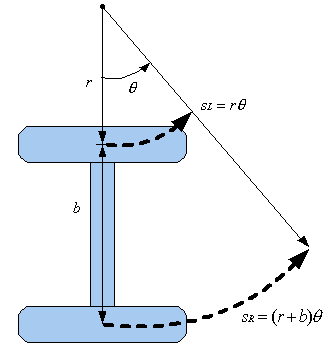
\includegraphics{diff_drive}
	\label{figDiffDrive}
\end{figure}

First, let's take a look at the standard theory for differential wheeled robots. Figure \ref{figDiffDrive} shows a simple two-wheeled robot making a left turn of \(\theta\) radians around some point. We assume the robot is one rigid body, and that each wheel maintains a constant velocity along the turn. This assumption of zero acceleration is obviously violated in the real world, but robots with a small mass and relatively powerful motors are able to approximate it well. \cite{differentialSteeringPaper}

\(r\) is the turning radius for the left wheel, and \((r+b)\) is the turning radius for the right wheel, where \(b\) is the distance between wheels. Using the formula for arc length, we know the distance traveled by the right and left wheels. Define a point M to be at the midpoint of the two wheels. This point will then travel an arc length of \((r+(b/2)) * \theta \). We can manipulate \(s_L\) and \(s_R\) to produce the following two equations.
\begin{equation} \label{eqDiffSM}
s_M = ((r+(b/2)) * \theta = (s_L + s_R) / 2
\end{equation}
\begin{equation} \label{eqDiffTheta}
\theta = (s_R - s_L) / b
\end{equation}

Equation \ref{eqDiffSM} gives the distance the center of the robot travels over the turn, in terms of the distance the two wheels traveled. Dividing this distance by the elapsed time it took to make the turn, gives an estimate of the instantaneous velocity of the robot at the end of the turn. Similarly, equation \ref{eqDiffTheta} calculates the angle of the turn using the distance the two wheels traveled. Dividing \(\theta\) by the elapsed time gives the angular velocity of the robot.

Both calculations make use of the distance traveled by the two wheels. The two quadrature motor encoders attached to the rover's front wheels give a certain number of counts per revolution, and the wheel circumference is given from the diameter. Thus the distance traveled can be surmised from the difference between the encoder ticks counted in the last sensor update, and those in the most recent update. This node uses these values to calculate the rover's angular and linear velocity. Only the angular velocity along the rover's z-axis is reported; the angular velocities along the other axes are assumed to be zero. Because a differentially steered robot can only move in the direction of its fixed wheels, the linear velocity is reported along the base\_link x axis, which faces forward from the rover's midpoint.

The Odometry message includes a six by six covariance matrix for the linear and angular velocities along all three axes. These covariances give the EKF node an idea of how much to trust these velocity estimates. Since only two velocities are calculated, reasonable constant variances squared for those two values are filled in along the matrix's diagonal. Every other element is set to zero, since they are ignored by the filter. 

Because dead reckoning estimates are naturally noisy and drift quickly, this project's EKF ignores the pose element of this node's Odometry message entirely. Therefore we don't bother with calculating the positional update estimate, or its covariance matrix.

This node is configured to publish Odometry messages at a rate equal to the Arduino's sensor update rate. If it published at a slower rate, then some resolution would be lost as the distance traveled is calculated from the difference between the most recent tick count, and the tick count used in the calculation of the prior Odometry estimate.

Though the number of encoder ticks per meter may be calculated from the encoders' specification and the diameter of the wheels, it is a good idea to manually calibrate the number of encoder ticks per meter, and pass this as a configurable parameter to this node. This helps account for sources of error. The ticks per meter can easily be calibrated by moving the Arduino one meter, while counting the number of encoder ticks.

\subsection{twist\_to\_motors}
Many ROS navigation packages produce Twist messages to command robotic platforms. The Twist message includes a linear and angular velocity, which the rover is expected to match, as a subfunction of some path following algorithm. The differential\_drive package uses the twist\_to\_motors node to translate Twist messages into individual motor velocities for each motor channel. 

Taking into account the differentially steered conditions, this node only considers the linear velocity along the rover's x axis, and the angular velocity around the rover's z-axis. Let's refer to these as \(x'\) and \(\theta '\), respectively. Let \(b\) once again be the distance between the rover's wheels. Let \(L'\) and \(R'\) be the velocity of the left and right wheels. From equation \ref{eqDiffSM}, we know that
\begin{equation*}
x' = (L' + R') / 2
\end{equation*}
and from equation \ref{eqDiffTheta} we know that
\begin{equation*}
\theta ' = (R' - L') / b
\end{equation*}

This is a system of two equations with two unknowns, \(L'\) and \(R'\). Solving this system gives us: 
\begin{multline*}
L' = x' - (b * \theta ') / 2 \\
R' = x' + (b * \theta ') / 2
\end{multline*}

This node performs this conversion, and publishes wheel velocities to the "lwheel\_vtarget" and "rwheel\_vtarget" topics. 

\subsection{pid\_velocity}
The pid\_velocity node creates a  proportional-integral-derivative (PID) controller which uses encoder feedback to translate motor velocities to actual motor R/C pulse commands. While the appropriate R/C servo command to reach a desired velocity could be estimated from the Sabertooth motor driver's datasheet, this would be the theoretical value and wouldn't take into account real-world sources of error such as uneven terrain, high traction, wind drag, etc. Therefore a control loop which utilizes real-time feedback is preferable.

Two of these nodes are run, one for each motor channel. One node subscribes to the topic "lwheel\_vtarget", and publishes commands to "/cmd/left", while the other node subscribes to "rwheel\_vtarget", and publishes to "/cmd/right". The Arduino node, through its bridge, is subscribed to these two topics and handles their messages appropriately.

PID controllers work by adjusting their output according an error term, which is the difference between the current feedback and the desired value. This error, the integral of all past error terms, and the estimated error of this derivative are all combined into a weighted sum. This sum then acts as the new output of the system.

This means that PID controllers have three parameters: \(K_p\), \(K_i\), and \(K_d\). These parameters must be manually tuned for optimal use of the controller. The tuning procedure involves zeroing out \(K_i\) and \(K_d\), and slowly increasing \(K_p\) until oscillation is observed in the control loop. Once a limit is found, set \(K_p\) to half of it. Then tune \(K_i\) and lastly \(K_d\), in the same fashion. 

\subsection{virtual\_joystick}
For manual driving of the rover, the differential\_drive package provides a joystick node, which brings up a simple GUI. This app allows the user to drag their mouse along a simple two-dimensional axis representing a desired linear and angular velocity, and publishes the corresponding Twist message. This is useful for manual testing of the rover, but will not needed once autonomous navigation is fully functional. This node requires installation of PySide, the python binding for the Qt framework.

\section{Ros Sensors App}
Android app to publish IMU and GPS data from a smartphone.

phone frame

\subsection{GPS}
GPS receivers background
coastguard broadcasts fix message for gps, don't have hardware to access that though

navsatfix message
covariance matrix

\subsection{IMU}
IMU chips background: magnetometers, accelerometers, gyroscopes
what a quaternion is

publishes IMU message

IMU messages are expected to be in ENU reference frame, instead of NED.

Android TYPE\_ROTATION\_VECTOR sensor fuses magnetometer and accelerometer data to produce an quaternion representation of an orientation in the ENU frame.

% https://source.android.com/devices/sensors/sensor-types#rotation_vector
Android accelometer readings tell us the linear acceleration of the rover, but are reported with respect to the local orientation of the phone, and so the node converts them to the ENU orientation before publishing them, in the phone frame (which just specifies a static translation)

Android gyroscope readings tell us the angular velocity of the rover, but are reported with respect to the local axes of the phone. However, our rover operates solely in 2D, and so we aren't interested in angular velocities of roll or pitch. And since the phone lays face-up on top of the rover, the phone's local z axis is the same as the ENU up axis, and so we don't need to transform the gyroscope reading for rad/sec rotation of yaw.



covariance matrices

\subsection{How to use}
usb tethering
on linux


\section{robot\_localization} \label{sectionRobotLocalization}
%http://docs.ros.org/kinetic/api/robot_localization/html/

package for state estimation

\cite{robot_localization_paper}

\subsection{Data Format Conventions}
REP-103 and REP-105 for conventions
true north, magnetic declination




\section{auto\_rover}
custom package
this is where custom message type, EncCount is defined, and header files are created
\subsection{EncCount} \label{sectionEncCount}

\subsection{range\_converter}
ping sensor at ultrasound frame

Adjust code for conversion of ultrasonic sensor ping times to distance, to take into account the ambient air temperature
If an echo has been received, then the speed of sound in air in m/s, \(C_{air}\), is calculated using the current air temperature in Celsius \(T_C\):
\[C_{air} = 331.5 + (0.6 * T_C)*\]

Multiplying \(C_{air}\) by the duration of the timed output pulse gives the estimated distance of the first object in front of the sensor.

Subscribes to /ping/timeUS and /ping/angleDeg topics, reads servo angle and ping time from those topics. Those messages sent from arduino to minimize amount of data being sent over serial. Then this node converts that to a distance in meters and an ultrasound -> base\_link transform. transform uses static translation from center of rover to center of PING))) sensor, as well as instantaneously changing rotation at each ping snapshot.

\subsection{}
First ekf\_localization node takes in odometry estimate from wheel encoders via diff\_odom node (section \ref{sectionOdomPublishing}), and IMU message from phone node. Produces a fused estimate of odometry.

navsat\_transform\_node takes in odometry message from first ekf node, which is the robot’s current position estimate in the frame specified by its start location. It also takes in the navsatfix and imu messages from the phone, and fuses all these to produce a different odometry estimate which is the gps data converted to the coordinates of the robot's world frame.

Second ekf\_localization node fuses the gps and odometry outputs from the previous two nodes into a final odometry message which is the final estimation of the robot's current state.


\cite{robot_localization_paper}